\documentclass[11pt,a4paper]{article}

\usepackage[utf8]{inputenc}
\usepackage[T1]{fontenc}
\usepackage{mathpazo}
\usepackage[scaled=0.92]{helvet}
\usepackage[margin=1in]{geometry}
\usepackage{graphicx}
\usepackage{amsmath,amssymb,amsfonts}
\usepackage{booktabs}
\usepackage{tabularx}
\usepackage{setspace}
\usepackage{titlesec}
\usepackage{fancyhdr}
\usepackage{float}
\usepackage{caption}
\usepackage{microtype}
\usepackage{tikz}
\usepackage{xcolor}
\usepackage{listings}
\usepackage[hidelinks]{hyperref}

\usetikzlibrary{shapes.geometric, arrows.meta, positioning, calc, matrix, fit, backgrounds}

\setstretch{1.15}
\setlength{\parindent}{0pt}
\setlength{\parskip}{0.8em}
\sloppy

\titleformat{\section}{\normalfont\large\bfseries\sffamily}{\thesection}{1em}{}
\titleformat{\subsection}{\normalfont\normalsize\bfseries\sffamily}{\thesubsection}{1em}{}
\titleformat{\subsubsection}{\normalfont\normalsize\itshape\sffamily}{\thesubsubsection}{1em}{}

\pagestyle{fancy}
\fancyhf{}
\fancyhead[L]{\small\sffamily SRS Document}
\fancyhead[R]{\small\sffamily\thepage}
\renewcommand{\headrulewidth}{0.4pt}

\captionsetup{font=small,labelfont=bf,labelsep=period}

\renewenvironment{abstract}
{\small
	\begin{center}\textbf{\sffamily Abstrak}\end{center}
	\begin{quote}}
	{\end{quote}}

\lstdefinestyle{code}{
	basicstyle=\ttfamily\small,
	frame=single,
	rulecolor=\color{black},
	breaklines=true,
	showstringspaces=false,
	columns=fullflexible,
	keepspaces=true,
	framesep=6pt,
	aboveskip=1em,
	belowskip=1em,
	xleftmargin=0pt
}

\lstdefinestyle{out}{
	basicstyle=\ttfamily\small,
	frame=tb,
	rulecolor=\color{black},
	breaklines=true,
	showstringspaces=false,
	columns=fullflexible,
	keepspaces=true,
	framesep=4pt,
	aboveskip=1em,
	belowskip=1em
}

\title{\vspace{-1.5cm}\textbf{\sffamily\LARGE Software Requirements Specification\\ Cetak Biru yang Tidak Boleh Ambigu}}
\author{
	\textbf{Muhammad Riduwan Khafidi} \\
	\small Program Studi Teknik Rekayasa Perangkat Lunak \\
	\small Politeknik Negeri Batam \\
	\small \texttt{4342611034@students.polibatam.ac.id}
}
\date{\small\today}

\begin{document}

\maketitle
\thispagestyle{empty}

\begin{abstract}
	Makalah ini membahas Software Requirements Specification sebagai dokumen yang berdiri di antara visi bisnis dan desain teknis. Ia menjelaskan perbedaan SRS dari dokumen lain, empat bab wajib beserta komponennya, template user story beserta kriteria penerimaan, sepuluh parameter non-fungsional yang lazim, dan lima langkah penulisan SRS yang bisa langsung dijalankan. Delapan visualisasi dan empat tabel menyertai pembahasan, termasuk tabel perbandingan bab, tabel kesalahan umum, dan lembar rujukan cepat. Sebuah studi kasus sepuluh langkah dengan aplikasi perpajakan startup mengikuti dokumen asli tapi menambahkan analisis yang tidak muncul di sana: mengapa setiap bagian ditulis dengan cara tertentu, siapa pembacanya, dan apa yang terjadi bila bagian itu dilewatkan. Paper ini juga menempatkan SRS pada posisi yang tepat dalam rantai dokumen requirement: setelah Vision and Scope, sebelum technical specification.
\end{abstract}

\section{Pendahuluan}

\subsection{Analogi Pembuka}

Bayangkan tiga profesi yang membangun rumah. Arsitek membuat gambar besar: bentuk rumah, jumlah kamar, posisi dapur. Insinyur sipil menerjemahkan gambar itu menjadi spesifikasi teknis: ketebalan balok, jenis besi, kadar semen, kedalaman pondasi. Tukang bangunan mengikuti spesifikasi teknis itu untuk memasang bata satu per satu.

Software Requirements Specification adalah spesifikasi teknis itu. Ia bukan gambar arsitek, tapi juga bukan instruksi pasang bata. Ia adalah dokumen yang menerjemahkan keinginan pemilik rumah menjadi kalimat yang bisa dieksekusi oleh tukang, dengan presisi yang cukup sehingga tukang tidak perlu menebak.

Kalau gambar arsitek diganti di tengah jalan, tukang berhenti dan menunggu. Kalau spesifikasi teknis diganti di tengah jalan, sebagian pekerjaan harus dibongkar. Itulah sebabnya spesifikasi teknis harus jelas sebelum pekerjaan dimulai, bukan setelahnya.

\subsection{Mengapa Topik Ini Penting}

Di minggu-minggu sebelumnya, kita mempelajari bagaimana menggali requirement, siapa stakeholder-nya, bagaimana membedakan empat tipe requirement, dan bagaimana menetapkan vision dan scope. Semua itu adalah \textbf{bahan mentah}. SRS adalah \textbf{produk jadinya}.

Tanpa SRS, pengembangan berjalan dari ingatan ke ingatan. Bug sering bukan karena kode salah, tapi karena tidak pernah ada dokumen yang disepakati tentang apa yang seharusnya dibangun. SRS adalah dokumen kesepakatan itu, ditulis pada level yang bisa diuji.

\subsection{Peta Pembahasan}

Makalah ini disusun berurutan. Bagian kedua menempatkan SRS pada rantai dokumen requirement. Bagian ketiga membahas empat bab wajib. Bagian keempat sampai ketujuh membahas satu per satu: BAB I Pendahuluan, BAB II Deskripsi Umum, BAB III Kebutuhan Spesifik, dan lampiran. Bagian kedelapan membahas user story. Bagian kesembilan membahas sepuluh parameter non-fungsional. Bagian kesepuluh membahas lima langkah penulisan SRS. Bagian kesebelas sampai ketiga belas merangkum perbandingan, kesalahan umum, dan lembar rujukan cepat. Bagian keempat belas memandu studi kasus sepuluh langkah dengan aplikasi perpajakan startup. Bagian kelima belas menutup dengan tiga prinsip.

\section{Posisi SRS pada Rantai Dokumen}

SRS bukan dokumen tunggal. Ia adalah salah satu dari tiga dokumen yang berjalan berurutan. Perhatikan Gambar~\ref{fig:doc-chain}.

\begin{figure}[H]
	\centering
	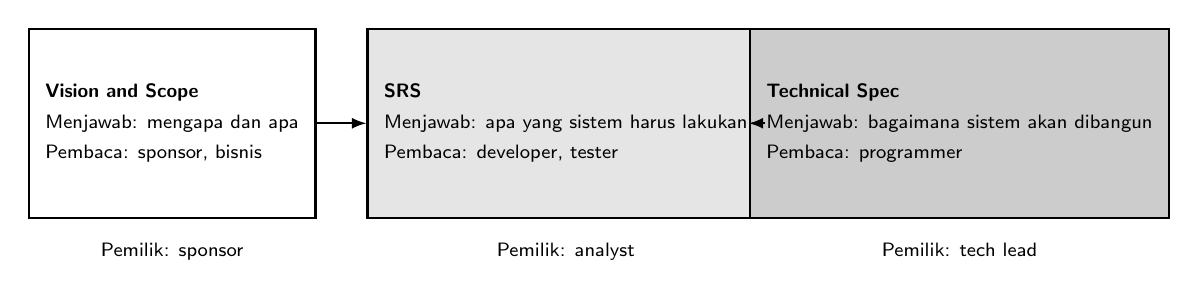
\begin{tikzpicture}[
			docbox/.style={rectangle, draw=black, thick, minimum width=3.4cm, minimum height=2.4cm, align=left, font=\sffamily\scriptsize, inner sep=6pt},
			arr/.style={draw, thick, -latex},
			owner/.style={font=\sffamily\scriptsize, anchor=north}
		]
		\node[docbox, fill=white] (vs) at (0, 0) {
			\textbf{Vision and Scope} \\[3pt]
			Menjawab: mengapa dan apa \\[3pt]
			Pembaca: sponsor, bisnis
		};
		\node[docbox, fill=black!10] (srs) at (5, 0) {
			\textbf{SRS} \\[3pt]
			Menjawab: apa yang sistem harus lakukan \\[3pt]
			Pembaca: developer, tester
		};
		\node[docbox, fill=black!20] (ts) at (10, 0) {
			\textbf{Technical Spec} \\[3pt]
			Menjawab: bagaimana sistem akan dibangun \\[3pt]
			Pembaca: programmer
		};

		\draw[arr] (vs.east) -- (srs.west);
		\draw[arr] (srs.east) -- (ts.west);

		\node[owner] at (0, -1.4) {Pemilik: sponsor};
		\node[owner] at (5, -1.4) {Pemilik: analyst};
		\node[owner] at (10, -1.4) {Pemilik: tech lead};
	\end{tikzpicture}
	\caption{Posisi SRS di antara Vision and Scope dan Technical Specification.}
	\label{fig:doc-chain}
\end{figure}

Tiga hal yang membedakan SRS dari dua dokumen lainnya.

\textbf{Pertama, pembacanya berbeda.} Vision and Scope dibaca sponsor untuk memutuskan apakah proyek ini layak dilanjutkan. SRS dibaca developer untuk memahami apa yang harus dibangun. Technical Spec dibaca programmer untuk memahami bagaimana membangunnya. Kalau SRS ditulis dengan bahasa sponsor, developer bingung. Kalau SRS ditulis dengan bahasa programmer, ia sudah jadi technical spec, bukan SRS.

\textbf{Kedua, isinya berbeda.} Vision and Scope berbicara tentang business opportunity, risiko, dan major features. SRS berbicara tentang input, proses, output, dan kriteria penerimaan. Technical Spec berbicara tentang arsitektur, database schema, dan pemilihan library.

\textbf{Ketiga, pemiliknya berbeda.} Vision and Scope dimiliki sponsor. SRS dimiliki analyst. Technical Spec dimiliki tech lead. Ketika sebuah keputusan harus diambil, yang berwenang adalah pemilik dokumen yang bersangkutan.

\section{Empat Bab Wajib}

SRS yang baik punya struktur yang konsisten. Dokumen contoh yang menjadi acuan paper ini mengikuti empat bab: tiga bab utama ditambah lampiran. Perhatikan Gambar~\ref{fig:four-chapters}.

\begin{figure}[H]
	\centering
	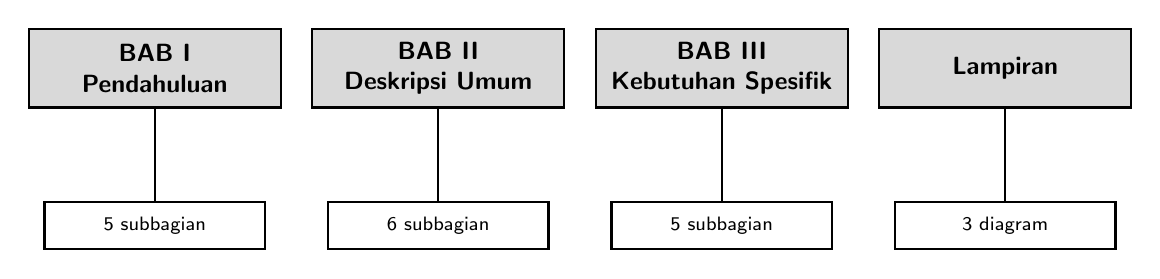
\begin{tikzpicture}[
			babbox/.style={rectangle, draw=black, thick, fill=black!15, minimum width=3.2cm, minimum height=1.0cm, align=center, font=\sffamily\small\bfseries},
			subbox/.style={rectangle, draw=black, thick, fill=white, minimum width=2.8cm, minimum height=0.6cm, align=center, font=\sffamily\scriptsize, inner sep=3pt},
			conn/.style={draw, thick}
		]
		\node[babbox] (b1) at (0, 0)   {BAB I\\Pendahuluan};
		\node[babbox] (b2) at (3.6, 0) {BAB II\\Deskripsi Umum};
		\node[babbox] (b3) at (7.2, 0) {BAB III\\Kebutuhan Spesifik};
		\node[babbox] (b4) at (10.8, 0) {Lampiran};

		\node[subbox] (s1) at (0, -2)    {5 subbagian};
		\node[subbox] (s2) at (3.6, -2)  {6 subbagian};
		\node[subbox] (s3) at (7.2, -2)  {5 subbagian};
		\node[subbox] (s4) at (10.8, -2) {3 diagram};

		\draw[conn] (b1.south) -- (s1.north);
		\draw[conn] (b2.south) -- (s2.north);
		\draw[conn] (b3.south) -- (s3.north);
		\draw[conn] (b4.south) -- (s4.north);
	\end{tikzpicture}
	\caption{Empat bab wajib SRS beserta jumlah subbagian tipikal.}
	\label{fig:four-chapters}
\end{figure}

\textbf{BAB I Pendahuluan} menjelaskan konteks dokumen: apa tujuan SRS, apa ruang lingkupnya, siapa yang harus membaca, apa istilah yang dipakai, dan referensi yang dirujuk.

\textbf{BAB II Deskripsi Umum} memberi gambaran tingkat tinggi produk: perspektif, fitur utama, manfaat, karakteristik pengguna, batasan, dan asumsi.

\textbf{BAB III Kebutuhan Spesifik} adalah inti SRS. Berisi kebutuhan fungsional, non-fungsional, antarmuka, user story, dan lingkungan operasi.

\textbf{Lampiran} berisi diagram dan artefak pelengkap: BPMN, usecase diagram, data flow diagram.

Urutan ini tidak boleh dibalik. Membaca SRS dari BAB III tanpa BAB I dan II akan membingungkan, karena pembaca tidak tahu konteks dokumen. Membaca dari BAB I tanpa BAB III akan mengecewakan, karena pembaca tidak mendapat informasi konkret.

\section{BAB I: Pendahuluan}

BAB I punya lima subbagian wajib. Perhatikan Gambar~\ref{fig:bab-one}.

\begin{figure}[H]
	\centering
	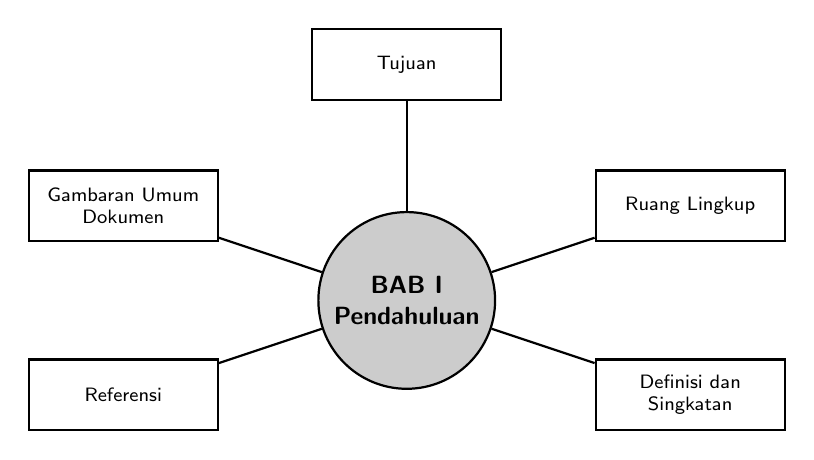
\begin{tikzpicture}[
			hub/.style={circle, draw=black, thick, fill=black!20, minimum size=1.6cm, align=center, font=\sffamily\small\bfseries},
			comp/.style={rectangle, draw=black, thick, fill=white, minimum width=2.4cm, minimum height=0.9cm, align=center, font=\sffamily\scriptsize, inner sep=3pt},
			conn/.style={draw, thick}
		]
		\node[hub] (c) at (0,0) {BAB I\\Pendahuluan};

		\node[comp] (c1) at (0, 3)    {Tujuan};
		\node[comp] (c2) at (3.6, 1.2) {Ruang Lingkup};
		\node[comp] (c3) at (3.6, -1.2) {Definisi dan\\Singkatan};
		\node[comp] (c4) at (-3.6, -1.2) {Referensi};
		\node[comp] (c5) at (-3.6, 1.2) {Gambaran Umum\\Dokumen};

		\draw[conn] (c) -- (c1);
		\draw[conn] (c) -- (c2);
		\draw[conn] (c) -- (c3);
		\draw[conn] (c) -- (c4);
		\draw[conn] (c) -- (c5);
	\end{tikzpicture}
	\caption{Lima subbagian wajib BAB I Pendahuluan.}
	\label{fig:bab-one}
\end{figure}

\textbf{Tujuan} menjelaskan mengapa SRS ini ditulis. Bukan mengapa proyek ini ada (itu tugas Vision and Scope), tapi mengapa dokumen panduan ini diperlukan. Contoh dari dokumen acuan: ``menjelaskan tujuan utama dari dokumen SRS ini, yakni memberikan panduan yang jelas untuk pengembangan perangkat lunak.''

\textbf{Ruang Lingkup} mencantumkan batasan area aplikasi: fitur apa yang dikerjakan dan tidak dikerjakan. Dokumen acuan menyebut lima fasilitas: pencatatan transaksi, e-faktur bulanan, penghitungan PPh Final, dokumen lampiran, dan ringkasan transaksi.

\textbf{Definisi, Istilah, dan Singkatan} menjelaskan istilah teknis yang dipakai. Dokumen acuan mendefinisikan SRS, IEEE, dan SSL. Tanpa bagian ini, pembaca yang tidak familiar dengan istilah akan tersesat di tengah dokumen.

\textbf{Referensi} mencantumkan sumber hukum, standar, atau dokumen yang dirujuk. Dokumen acuan merujuk ke Standar IEEE 1058.1-1987 dan Peraturan Pemerintah No 46 Tahun 2013.

\textbf{Gambaran Umum Dokumen} memberi peta empat bab yang akan dibaca. Ini bagian yang sering dilewatkan, padahal ia berfungsi seperti daftar isi yang memberi tahu pembaca apa yang akan ia temukan di bab mana.

BAB I mungkin terasa administratif. Tapi ia yang menentukan apakah SRS ini bisa dibaca orang lain yang tidak terlibat dalam penulisannya. Tanpa BAB I, SRS hanya bisa dipahami oleh penulisnya sendiri.

\section{BAB II: Deskripsi Umum}

BAB II punya enam subbagian wajib. Perhatikan Gambar~\ref{fig:bab-two}.

\begin{figure}[H]
	\centering
	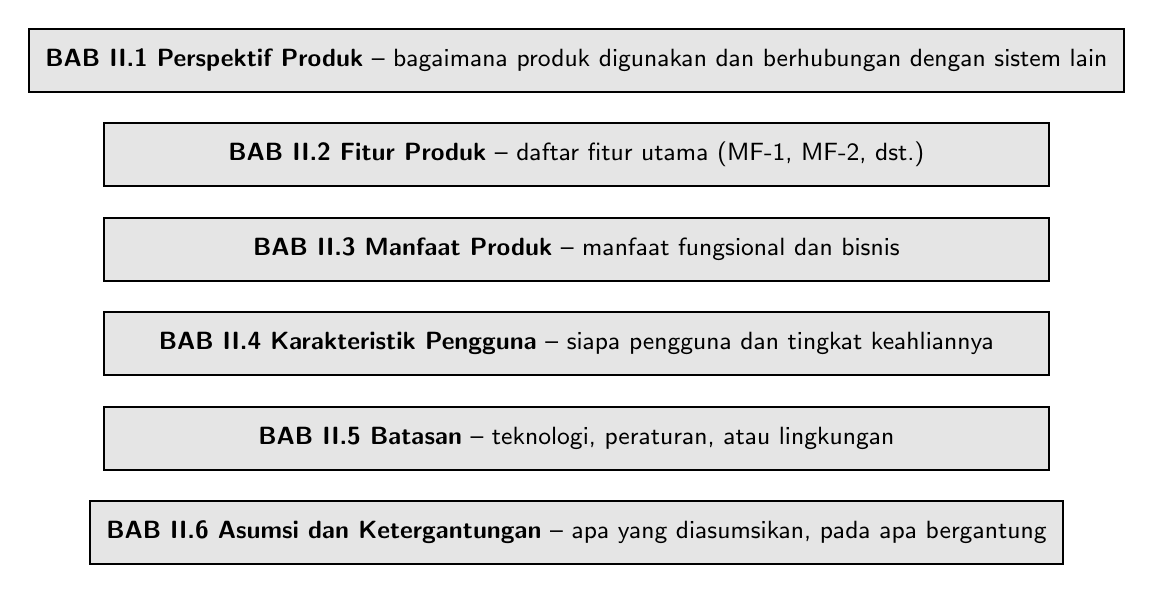
\begin{tikzpicture}[
			babrow/.style={rectangle, draw=black, thick, fill=black!10, minimum width=12cm, minimum height=0.8cm, align=left, font=\sffamily\small, inner sep=6pt}
		]
		\node[babrow] (b1) at (0,  3.6) {\textbf{BAB II.1 Perspektif Produk} -- bagaimana produk digunakan dan berhubungan dengan sistem lain};
		\node[babrow] (b2) at (0,  2.4) {\textbf{BAB II.2 Fitur Produk} -- daftar fitur utama (MF-1, MF-2, dst.)};
		\node[babrow] (b3) at (0,  1.2) {\textbf{BAB II.3 Manfaat Produk} -- manfaat fungsional dan bisnis};
		\node[babrow] (b4) at (0,  0)   {\textbf{BAB II.4 Karakteristik Pengguna} -- siapa pengguna dan tingkat keahliannya};
		\node[babrow] (b5) at (0, -1.2) {\textbf{BAB II.5 Batasan} -- teknologi, peraturan, atau lingkungan};
		\node[babrow] (b6) at (0, -2.4) {\textbf{BAB II.6 Asumsi dan Ketergantungan} -- apa yang diasumsikan, pada apa bergantung};
	\end{tikzpicture}
	\caption{Enam subbagian wajib BAB II Deskripsi Umum.}
	\label{fig:bab-two}
\end{figure}

\textbf{Perspektif Produk} menjelaskan bagaimana produk akan digunakan dan berhubungan dengan sistem lain. Dokumen acuan menyebut: produk dijalankan oleh pengguna dengan koneksi internet, dapat berjalan di platform apa saja yang mendukung aplikasi web.

\textbf{Fitur Produk} mendaftar fitur utama dengan kode (MF-1, MF-2, dst.) agar bisa dirujuk di bab berikutnya. Dokumen acuan mendaftar enam fitur: login/registrasi, pencatatan transaksi, e-faktur bulanan, hitung PPh Final, dokumen lampiran, dan ringkasan transaksi.

\textbf{Manfaat Produk} menjelaskan manfaat fungsional dan bisnis. Dokumen acuan menyebut tiga: memudahkan perpajakan PP 46/2013, mengurangi waktu pencatatan, menyediakan lampiran.

\textbf{Karakteristik Pengguna} menjelaskan pengguna dan tingkat keahlian yang dibutuhkan. Dokumen acuan membedakan dua peran: pemilik startup (akses penuh) dan staff keuangan (akses terbatas).

\textbf{Batasan} mencantumkan teknologi, peraturan, atau batasan lingkungan. Dokumen acuan menyebut lima batasan: mengikuti PP 46/2013, tidak menangani submission SPT, tidak menangani pembayaran ke bank, akses harus online, browser harus menerima SSL.

\textbf{Asumsi dan Ketergantungan} mencantumkan asumsi yang dipakai dan ketergantungan pada faktor eksternal. Dokumen acuan menyebut: bisa diakses dari mana saja via browser, dikembangkan dengan Platform as a Service.

Pembeda terpenting antara BAB II dan BAB III adalah level detail. BAB II berbicara tentang \textbf{kategori}, BAB III berbicara tentang \textbf{individual requirement}. BAB II menyebut ``enam fitur utama'', BAB III menjelaskan input dan output setiap fitur.

\section{BAB III: Kebutuhan Spesifik}

BAB III adalah inti SRS. Ia punya lima subbagian yang saling mengunci. Perhatikan Gambar~\ref{fig:bab-three}.

\begin{figure}[H]
	\centering
	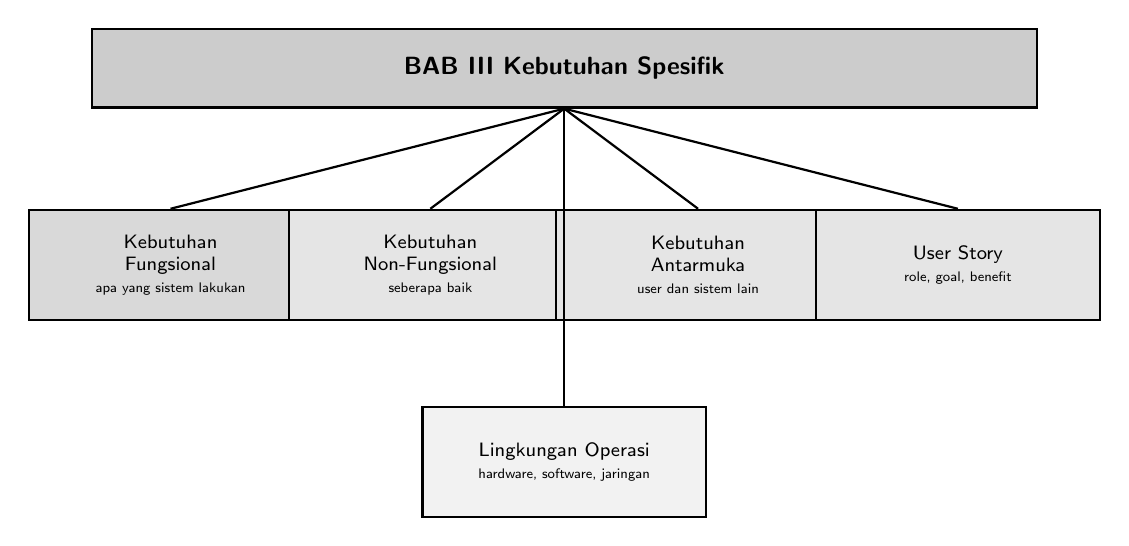
\begin{tikzpicture}[
			mainbox/.style={rectangle, draw=black, thick, fill=black!20, minimum width=12cm, minimum height=1.0cm, align=center, font=\sffamily\small\bfseries},
			subbox/.style={rectangle, draw=black, thick, fill=white, minimum width=3.6cm, minimum height=1.4cm, align=center, font=\sffamily\scriptsize, inner sep=4pt},
			conn/.style={draw, thick}
		]
		\node[mainbox] (main) at (0, 3.5) {BAB III Kebutuhan Spesifik};

		\node[subbox, fill=black!15] (s1) at (-5, 1) {Kebutuhan\\Fungsional\\{\tiny apa yang sistem lakukan}};
		\node[subbox, fill=black!10] (s2) at (-1.7, 1) {Kebutuhan\\Non-Fungsional\\{\tiny seberapa baik}};
		\node[subbox, fill=black!10] (s3) at (1.7, 1) {Kebutuhan\\Antarmuka\\{\tiny user dan sistem lain}};
		\node[subbox, fill=black!10] (s4) at (5, 1) {User Story\\{\tiny role, goal, benefit}};

		\node[subbox, fill=black!5] (s5) at (0, -1.5) {Lingkungan Operasi\\{\tiny hardware, software, jaringan}};

		\draw[conn] (main.south) -- (s1.north);
		\draw[conn] (main.south) -- (s2.north);
		\draw[conn] (main.south) -- (s3.north);
		\draw[conn] (main.south) -- (s4.north);
		\draw[conn] (main.south) -- (s5.north);
	\end{tikzpicture}
	\caption{Lima subbagian BAB III Kebutuhan Spesifik.}
	\label{fig:bab-three}
\end{figure}

\textbf{Kebutuhan Fungsional} mendaftar perilaku yang harus sistem lakukan. Dokumen acuan menyebut enam fungsi: pendaftaran, input transaksi, tampil e-faktur, hitung PPh Final, sediakan dokumen unduhan, sediakan ringkasan transaksi. Setiap fungsi diberi kode (FR-1, FR-2, dst.) agar bisa dilacak.

\textbf{Kebutuhan Non-Fungsional} mendaftar kualitas yang harus dipenuhi sistem. Dokumen acuan menyusunnya dalam tabel: Availability, Reliability, Ergonomy, Portability, Memory, Response Time, Safety, Security, dan Bahasa. Bagian ini dibahas lebih dalam di Bagian~\ref{sec:nfr}.

\textbf{Kebutuhan Antarmuka} menjelaskan antarmuka yang harus disediakan, baik untuk pengguna maupun sistem lain. Dokumen acuan membedakan hardware (PC, LAN card) dan software (browser).

\textbf{User Story} merumuskan kebutuhan dari sudut pandang pengguna. Dokumen acuan memakai format role-goal-benefit untuk setiap fitur MF-1 sampai MF-6. Bagian ini dibahas lebih dalam di Bagian~\ref{sec:user-story}.

\textbf{Lingkungan Operasi} mencantumkan platform, framework, dan bahasa yang dipakai. Dokumen acuan menyebut Visio 2016 untuk UML, Git dan Google Cloud SDK untuk cloud, PHP dan HTML untuk bahasa, MySQL untuk database.

Lima subbagian ini bekerja bersama. Functional requirement menjelaskan \textit{apa}. Non-functional menjelaskan \textit{seberapa baik}. Antarmuka menjelaskan \textit{di mana}. User story menjelaskan \textit{untuk siapa}. Lingkungan operasi menjelaskan \textit{dengan alat apa}. Melewatkan salah satunya menghasilkan SRS yang tidak lengkap.

\section{User Story}

\label{sec:user-story}

User story adalah cara merumuskan requirement dari sudut pandang pengguna. Ia punya struktur tetap yang memaksa penulis menjawab tiga pertanyaan sekaligus. Perhatikan Gambar~\ref{fig:user-story}.

\begin{figure}[H]
	\centering
	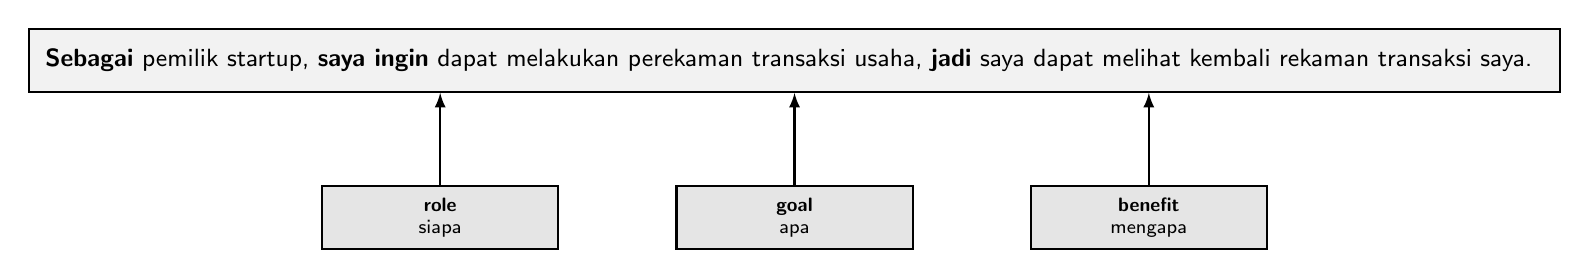
\begin{tikzpicture}[
			storybox/.style={rectangle, draw=black, thick, fill=white, minimum width=13cm, minimum height=0.8cm, align=left, font=\sffamily\small, inner sep=6pt},
			part/.style={rectangle, draw=black, thick, fill=black!10, minimum width=3cm, minimum height=0.8cm, align=center, font=\sffamily\scriptsize, inner sep=3pt}
		]
		\node[storybox, fill=black!5] (story) at (0, 2) {
			\textbf{Sebagai} pemilik startup, \textbf{saya ingin} dapat melakukan perekaman transaksi usaha, \textbf{jadi} saya dapat melihat kembali rekaman transaksi saya.
		};

		\node[part] (role) at (-4.5, 0) {\textbf{role}\\siapa};
		\node[part] (goal) at (0, 0)    {\textbf{goal}\\apa};
		\node[part] (benefit) at (4.5, 0) {\textbf{benefit}\\mengapa};

		\draw[thick, -latex] (role.north) -- (role.north |- story.south);
		\draw[thick, -latex] (goal.north) -- (goal.north |- story.south);
		\draw[thick, -latex] (benefit.north) -- (benefit.north |- story.south);
	\end{tikzpicture}
	\caption{Anatomi user story dengan tiga bagian wajib.}
	\label{fig:user-story}
\end{figure}

Struktur ini memaksa penulis menjawab tiga pertanyaan. Kalau salah satu tidak dijawab, user story menjadi kabur. Kalimat seperti ``sistem harus menyediakan fitur e-faktur'' bukan user story, karena tidak menjelaskan \textbf{siapa} yang memakai dan \textbf{mengapa} fitur itu penting.

User story saja tidak cukup. Ia harus dilengkapi \textbf{kriteria penerimaan}. Dokumen acuan menyebut kriteria seperti: pengguna harus melengkapi semua input yang diperlukan, informasi disimpan ke database, pengguna dapat melihat rekaman transaksi.

Kriteria penerimaan inilah yang membuat user story bisa diuji. Tanpa kriteria, user story hanya kalimat harapan. Dengan kriteria, user story menjadi kontrak yang bisa diverifikasi oleh QA.

\section{Kebutuhan Non-Fungsional}

\label{sec:nfr}

Kebutuhan non-fungsional menjelaskan \textit{seberapa baik} sistem harus bekerja. Dokumen acuan menyusunnya dalam tabel parameter. Perhatikan Gambar~\ref{fig:nfr-params}.

\begin{figure}[H]
	\centering
	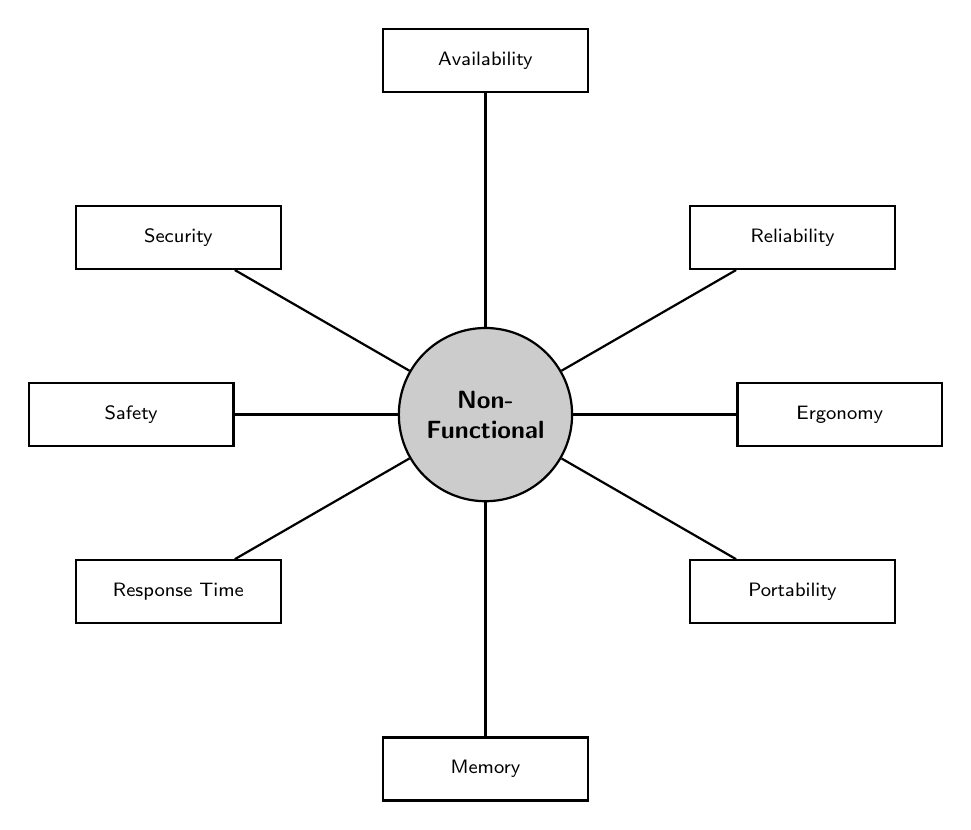
\begin{tikzpicture}[
			hub/.style={circle, draw=black, thick, fill=black!20, minimum size=2.2cm, align=center, font=\sffamily\small\bfseries},
			param/.style={rectangle, draw=black, thick, fill=white, minimum width=2.6cm, minimum height=0.8cm, align=center, font=\sffamily\scriptsize, inner sep=3pt},
			conn/.style={draw, thick}
		]
		\node[hub] (c) at (0,0) {Non-\\Functional};

		\node[param] (p1) at (0,    4.5) {Availability};
		\node[param] (p2) at (3.9,  2.25) {Reliability};
		\node[param] (p3) at (4.5,  0)    {Ergonomy};
		\node[param] (p4) at (3.9, -2.25) {Portability};
		\node[param] (p5) at (0,   -4.5)  {Memory};
		\node[param] (p6) at (-3.9,-2.25) {Response Time};
		\node[param] (p7) at (-4.5, 0)    {Safety};
		\node[param] (p8) at (-3.9, 2.25) {Security};

		\draw[conn] (c) -- (p1);
		\draw[conn] (c) -- (p2);
		\draw[conn] (c) -- (p3);
		\draw[conn] (c) -- (p4);
		\draw[conn] (c) -- (p5);
		\draw[conn] (c) -- (p6);
		\draw[conn] (c) -- (p7);
		\draw[conn] (c) -- (p8);
	\end{tikzpicture}
	\caption{Sembilan parameter non-fungsional yang lazim dicantumkan di SRS.}
	\label{fig:nfr-params}
\end{figure}

Dokumen acuan menyusun tabel parameter dengan requirement sebagai berikut.

\textbf{Availability}: sistem berjalan 24 jam non-stop kecuali ada perawatan atau pembaharuan. \textbf{Reliability}: kegagalan yang ditolerir sekitar 5 persen. \textbf{Ergonomy}: sistem user friendly. \textbf{Portability}: dapat diakses di platform apa saja yang menjalankan web. \textbf{Memory}: minimum 1024 MB. \textbf{Response Time}: tidak lebih dari 3 detik. \textbf{Safety}: browser harus menerima SSL. \textbf{Security}: akses online, offline tidak dilayani. \textbf{Bahasa}: menggunakan bahasa Indonesia.

Dari sembilan parameter ini, hanya satu yang punya angka presisi: Response Time (3 detik) dan Memory (1024 MB). Tujuh lainnya masih kualitatif. Ini contoh nyata dari prinsip yang sudah dibahas di minggu keempat: \textbf{non-functional requirement tanpa angka sulit diverifikasi}.

Untuk memperbaiki tabel seperti ini, ubah setiap parameter kualitatif menjadi angka. ``Reliability 5 persen'' bisa diperjelas menjadi ``sistem boleh gagal maksimal 5 persen request per bulan, diukur dengan uptime monitoring''. ``User friendly'' bisa diperjelas menjadi ``pengguna baru bisa menyelesaikan registrasi dalam kurang dari 3 menit tanpa panduan''. ``Bahasa Indonesia'' bisa diperjelas menjadi ``semua label, pesan error, dan notifikasi ditulis dalam bahasa Indonesia baku''.

\section{Lima Langkah Menulis SRS}

SRS yang baik ditulis dalam lima langkah berurutan. Perhatikan Gambar~\ref{fig:writing-flow}.

\begin{figure}[H]
	\centering
	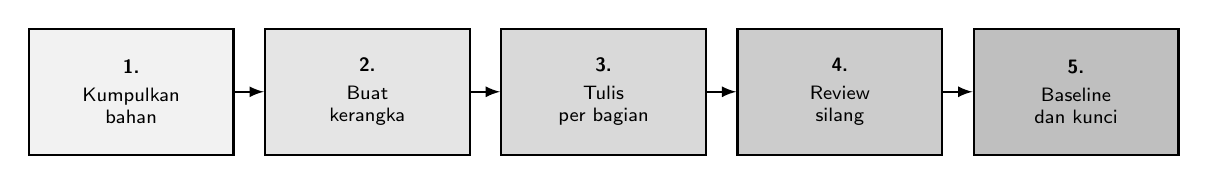
\begin{tikzpicture}[
			stepbox/.style={rectangle, draw=black, thick, fill=black!10, minimum width=2.6cm, minimum height=1.6cm, align=center, font=\sffamily\scriptsize, inner sep=3pt},
			arr/.style={draw, thick, -latex}
		]
		\node[stepbox, fill=black!5]  (s1) at (0, 0)    {\textbf{1.}\\[2pt]Kumpulkan\\bahan};
		\node[stepbox, fill=black!10] (s2) at (3, 0)    {\textbf{2.}\\[2pt]Buat\\kerangka};
		\node[stepbox, fill=black!15] (s3) at (6, 0)    {\textbf{3.}\\[2pt]Tulis\\per bagian};
		\node[stepbox, fill=black!20] (s4) at (9, 0)    {\textbf{4.}\\[2pt]Review\\silang};
		\node[stepbox, fill=black!25] (s5) at (12, 0)   {\textbf{5.}\\[2pt]Baseline\\dan kunci};

		\draw[arr] (s1) -- (s2);
		\draw[arr] (s2) -- (s3);
		\draw[arr] (s3) -- (s4);
		\draw[arr] (s4) -- (s5);
	\end{tikzpicture}
	\caption{Lima langkah penulisan SRS.}
	\label{fig:writing-flow}
\end{figure}

\textbf{Langkah 1: Kumpulkan bahan.} Ambil semua hasil elicitation dari minggu kedua: wawancara, observasi, kuesioner. Ambil dokumen Vision and Scope dari minggu kelima. Ambil dokumen requirement dari minggu keempat. Tanpa bahan ini, SRS akan berisi asumsi.

\textbf{Langkah 2: Buat kerangka.} Sebelum menulis satu kalimat pun, buat kerangka empat bab. Isi setiap bab dengan subbagian wajib. Kerangka ini mencegah penulis melompat-lompat.

\textbf{Langkah 3: Tulis per bagian.} Tulis BAB I dulu, lalu BAB II, lalu BAB III, terakhir lampiran. Jangan menulis BAB III dulu karena terasa paling penting. Pembaca akan membaca berurutan, jadi penulis harus menulis berurutan.

\textbf{Langkah 4: Review silang.} Minta tiga orang membaca: satu analyst lain (untuk konsistensi), satu developer (untuk kejelasan teknis), satu sponsor (untuk kesesuaian bisnis). Setiap reviewer fokus pada satu aspek.

\textbf{Langkah 5: Baseline dan kunci.} Setelah disetujui, kunci dokumen dan beri nomor versi. Setiap perubahan setelah baseline harus melalui change request, seperti yang sudah dibahas di minggu kelima.

\section{Perbandingan Ringkasan}

Tabel~\ref{tab:summary} merangkum empat bab dan fungsinya.

\begin{table}[H]
	\centering
	\caption{Ringkasan empat bab SRS dan fungsinya.}
	\label{tab:summary}
	\footnotesize
	\begin{tabularx}{\textwidth}{l X X}
		\toprule
		Bab                        & Pertanyaan yang Dijawab                   & Pembaca Utama           \\
		\midrule
		BAB I Pendahuluan          & Mengapa dokumen ini ada, siapa pembacanya & Semua pembaca baru      \\
		BAB II Deskripsi Umum      & Gambaran besar produk                     & Sponsor, calon pengguna \\
		BAB III Kebutuhan Spesifik & Apa yang sistem harus lakukan             & Developer, tester       \\
		Lampiran                   & Diagram pelengkap                         & Developer, auditor      \\
		\bottomrule
	\end{tabularx}
\end{table}

\section{Studi Kasus: Menyusun SRS Aplikasi Perpajakan}

Bagian ini memandu sepuluh langkah untuk menyusun SRS dengan contoh aplikasi perpajakan startup yang mengikuti PP 46/2013. Setiap langkah menghasilkan blok keluaran yang bisa langsung dipakai sebagai template.

\subsection{Langkah 1: Tulis BAB I.1 Tujuan}

Mulai dengan alasan mengapa dokumen SRS ini ditulis.

\begin{lstlisting}[style=out]
BAB I.1 Tujuan:

Dokumen SRS ini memberikan panduan yang jelas bagi
tim pengembangan aplikasi perpajakan bagi startup,
sehingga setiap fitur yang dibangun dapat dilacak
ke requirement yang sudah disepakati.

Perusahaan rintisan atau startup memiliki kekurangan
pemahaman tentang PP 46 Tahun 2013, sehingga
mengalami kesulitan dalam perhitungan dan pelaporan
pajak. Pencatatan keuangan dan pelaporan pajak masih
terpisah dan manual.

Aplikasi ini akan melakukan pencatatan transaksi,
membantu perhitungan pajak, dan menyediakan lampiran
transaksi yang sudah direkam.
\end{lstlisting}

\subsection{Langkah 2: Tulis BAB I.2 Ruang Lingkup}

Batasi area yang dikerjakan dan yang tidak.

\begin{lstlisting}[style=out]
BAB I.2 Ruang Lingkup:

Termasuk dalam lingkup:
1. Sistem melayani pencatatan transaksi usaha.
2. Sistem menyediakan fitur e-faktur bulanan.
3. Sistem menghitung PPh Final bulanan dan tahunan.
4. Sistem memberikan dokumen yang dapat diunduh
   sebagai lampiran.
5. Sistem memberikan ringkasan transaksi usaha.

Tidak termasuk dalam lingkup:
- Proses submission laporan SPT ke Dirjen Pajak.
- Proses pembayaran pajak ke bank.
- Akses offline.
\end{lstlisting}

\subsection{Langkah 3: Tulis BAB II.2 Fitur Produk}

Daftar fitur dengan kode agar bisa dirujuk.

\begin{lstlisting}[style=out]
BAB II.2 Fitur Produk:

MF-1: Menyediakan menu login dan registrasi bagi
      startup.
MF-2: Melayani pencatatan transaksi usaha.
MF-3: Menyediakan fitur e-faktur bulanan.
MF-4: Menghitung PPh Final Tahunan pada startup.
MF-5: Memberikan dokumen yang dapat diunduh
      sebagai lampiran.
MF-6: Memberikan ringkasan transaksi usaha.

Setiap fitur akan dijabarkan lebih lanjut di BAB III
sebagai functional requirement, dan di bagian User
Story sebagai role-goal-benefit.
\end{lstlisting}

\subsection{Langkah 4: Tulis BAB II.4 Karakteristik Pengguna}

Bedakan pengguna berdasarkan akses dan tanggung jawab.

\begin{lstlisting}[style=out]
BAB II.4 Karakteristik Pengguna:

1. Pemilik startup atau UKM/UMKM
   - Akses terhadap seluruh fitur
   - Mengelola staff yang dapat mengakses fitur
   - Melihat laporan dan ringkasan transaksi

2. Staff keuangan pada startup
   - Akses terbatas sesuai yang diatur pemilik
   - Dapat melakukan pencatatan transaksi
   - Dapat melihat perhitungan PPh Final
   - Dapat melakukan penyetoran

Perbedaan akses harus diterapkan di level
autentikasi dan otorisasi, bukan hanya
disembunyikan dari antarmuka.
\end{lstlisting}

\subsection{Langkah 5: Tulis BAB III Kebutuhan Fungsional}

Turunkan setiap fitur MF menjadi functional requirement.

\begin{lstlisting}[style=out]
BAB III Kebutuhan Fungsional:

FR-1: Pendaftaran pengguna
Deskripsi: Merekam data lengkap pengguna untuk
keperluan administrasi sistem.
Input: nama, email, password, nama usaha.
Output: akun pengguna aktif dengan role default.

FR-2: Input transaksi usaha atau faktur
Deskripsi: Merekam transaksi usaha yang dapat
berupa satu atau beberapa transaksi dalam satu
faktur.
Input: nomor faktur, tanggal, jumlah, nama
pembeli, deskripsi.
Output: rekaman faktur di database.

FR-3: Menampilkan rekaman e-faktur bulanan
Deskripsi: Menampilkan daftar faktur yang sudah
direkam, dengan opsi ubah dan hapus.
Input: filter bulan dan tahun.
Output: daftar faktur beserta aksi.

FR-4: Perhitungan PPh Final bulanan dan tahunan
Deskripsi: Menghitung PPh Final 1 persen dari
total peredaran bruto bulanan, dan rangkuman
tahunan.
Input: data faktur yang sudah direkam.
Output: nominal PPh Final bulanan dan tahunan.

FR-5: Dokumen lampiran
Deskripsi: Membuat dokumen laba/rugi dan daftar
peredaran bruto sebagai lampiran SPT Tahunan.
Input: data transaksi satu tahun pajak.
Output: dokumen unduhan berformat PDF.

FR-6: Ringkasan transaksi usaha
Deskripsi: Membuat ringkasan transaksi yang
dikirim berkala ke pemilik usaha.
Input: seluruh transaksi yang sudah direkam.
Output: ringkasan transaksi bulanan.
\end{lstlisting}

\subsection{Langkah 6: Tulis BAB III Kebutuhan Non-Fungsional}

Ubah setiap parameter menjadi angka yang bisa diuji.

\begin{lstlisting}[style=out]
BAB III Kebutuhan Non-Fungsional (versi diperbaiki):

NFR-1 (Availability): Sistem berjalan 24 jam
non-stop, di luar jadwal pemeliharaan terjadwal,
dengan uptime minimal 99,5 persen per bulan.

NFR-2 (Reliability): Kegagalan request yang
ditolerir maksimal 5 persen per bulan, diukur
dengan uptime monitoring.

NFR-3 (Ergonomy): Pengguna baru dapat
menyelesaikan registrasi dalam kurang dari 3
menit tanpa panduan tertulis.

NFR-4 (Portability): Sistem berjalan di Chrome,
Firefox, Safari, dan Edge versi terbaru.

NFR-5 (Memory): Server minimum 1024 MB RAM per
instance aplikasi.

NFR-6 (Response Time): 95 persen request
diselesaikan dalam waktu kurang dari 3 detik.

NFR-7 (Safety): Semua koneksi menggunakan SSL
dengan sertifikat valid.

NFR-8 (Security): Password disimpan dengan hash
bcrypt. Sesi berakhir setelah 30 menit idle.
Akses offline tidak dilayani.

NFR-9 (Bahasa): Semua label, pesan error, dan
notifikasi menggunakan bahasa Indonesia baku.
\end{lstlisting}

\subsection{Langkah 7: Tulis BAB III User Story dengan Kriteria Penerimaan}

Setiap fitur MF punya satu user story dengan kriteria.

\begin{lstlisting}[style=out]
BAB III User Story MF-2 (Input Transaksi):

User Story:
Sebagai pemilik startup, saya ingin dapat melakukan
perekaman transaksi usaha, jadi saya dapat melihat
kembali rekaman transaksi saya.

Kriteria Penerimaan:
1. Pengguna harus melengkapi nomor faktur,
   tanggal, jumlah, dan nama pembeli.
2. Nomor faktur harus unik per tahun pajak.
3. Seluruh rekaman transaksi tersimpan di database
   dengan timestamp pembuatan.
4. Pengguna dapat melihat rekaman transaksi di
   halaman daftar faktur.

BAB III User Story MF-4 (Perhitungan PPh Final):

User Story:
Sebagai pemilik startup, saya ingin perhitungan
pajak PPh Final dapat dilakukan otomatis, jadi
saya bisa mendapatkan hasilnya secara langsung.

Kriteria Penerimaan:
1. Perhitungan hanya berjalan setelah ada minimal
   satu transaksi bulan tersebut.
2. PPh Final dihitung 1 persen dari total
   peredaran bruto bulanan.
3. Hasil ditampilkan dalam format Rupiah dengan
   dua angka desimal.
\end{lstlisting}

\subsection{Langkah 8: Tulis BAB III Kebutuhan Antarmuka}

Bedakan antarmuka hardware dan software.

\begin{lstlisting}[style=out]
BAB III Kebutuhan Antarmuka:

Hardware Interface:
- Perangkat PC dengan CPU, mouse, keyboard, dan
  monitor.
- LAN Card untuk koneksi ke jaringan internet.
- Server VPS di Google Cloud Platform dengan
  spesifikasi 4 vCPU, 8 GB RAM, 500 GB disk.

Software Interface:
- Browser: Chrome, Firefox, Safari, atau Edge
  versi terbaru.
- Komponen antarmuka: label, textbox, combobox,
  button, table.
- Protokol: HTTPS dengan SSL untuk keamanan.

Prototipe Antarmuka:
1. Halaman Rekam Transaksi (pola dua kolom:
   form di kanan, daftar faktur di kiri).
2. Halaman Daftar Rekam Faktur dengan ringkasan
   PPh Final 1 persen.
3. Halaman Setor Pajak Final dengan status
   pembayaran per masa pajak.
4. Halaman Generate Lampiran SPT dalam bentuk
   tabel peredaran bruto.
\end{lstlisting}

\subsection{Langkah 9: Tulis Lampiran}

Sertakan tiga diagram wajib.

\begin{lstlisting}[style=out]
Lampiran SRS:

Lampiran 1: Business Process Model (BPMN)
- Sebelum: proses pajak manual oleh startup,
  bank, dan Dirjen Pajak.
- Sesudah: proses dengan aplikasi yang mengotomasi
  perhitungan, tapi pembayaran dan pelaporan SPT
  tetap manual.

Lampiran 2: Use Case Diagram
- Aktor: Pemilik startup, Staff keuangan.
- Use case: mendaftar, merekam transaksi,
  menghitung pajak PPh Final, me-generate
  lampiran/dokumen.

Lampiran 3: Data Flow Diagram
- Proses 1: Pendaftaran (input: nama, no_hp, sandi;
  output: tabel tb_customer).
- Proses 2: Rekam transaksi (output: tabel tb_faktur).
- Proses 3: Perhitungan PPh Final (output: tabel
  tb_pajak_final).
- Proses 4: Generate dokumen (output: file PDF).
\end{lstlisting}

\subsection{Langkah 10: Review Silang dan Baseline}

Sebelum mengunci dokumen, lakukan tiga review.

\begin{lstlisting}[style=out]
Checklist Review Silang:

Review 1 - Konsistensi (oleh analyst lain):
- Setiap FR melacak ke satu MF.
- Setiap MF punya minimal satu user story.
- Tidak ada istilah yang dipakai berbeda di dua
  bagian.
- Semua singkatan sudah didefinisikan di BAB I.3.

Review 2 - Kejelasan Teknis (oleh developer):
- Setiap FR punya input, proses, dan output.
- Setiap NFR punya angka atau kriteria uji.
- Antarmuka hardware dan software jelas.

Review 3 - Kesesuaian Bisnis (oleh sponsor):
- Ruang lingkup sesuai dengan visi dan scope.
- Batasan dan asumsi wajar.
- Manfaat produk sesuai dengan target bisnis.

Setelah ketiga review selesai, dokumen diberi
nomor versi 1.0 dan dikunci. Setiap perubahan
setelah ini harus melalui change request.
\end{lstlisting}

Sepuluh langkah di atas menghasilkan tiga artefak siap kumpul: dokumen SRS lengkap empat bab, prototipe antarmuka empat halaman, dan tiga diagram lampiran (BPMN, use case, DFD). Inilah deliverable SRS.

\section{Kesalahan Umum}

Tabel~\ref{tab:mistakes} merangkum kesalahan yang paling sering muncul saat menulis SRS.

\begin{table}[H]
	\centering
	\caption{Kesalahan umum pada penulisan SRS.}
	\label{tab:mistakes}
	\footnotesize
	\begin{tabularx}{\textwidth}{l X X}
		\toprule
		Kesalahan                            & Akibat                                       & Perbaikan                                          \\
		\midrule
		Melewatkan BAB I                     & Pembaca baru bingung, istilah tidak jelas    & Selalu tulis BAB I meskipun terasa administratif   \\
		Menulis SRS dengan bahasa teknis     & Sponsor tidak bisa review                    & Tulis di level perilaku, bukan implementasi        \\
		Menulis SRS dengan bahasa bisnis     & Developer tidak bisa mengeksekusi            & Setiap FR harus punya input, proses, output        \\
		Non-functional tanpa angka           & Tidak bisa diverifikasi                      & Ganti ``user friendly'' dengan angka terukur       \\
		User story tanpa kriteria penerimaan & Tidak bisa diuji                             & Setiap user story minimal punya 2 kriteria         \\
		Functional requirement tanpa kode    & Tidak bisa dilacak ke user story dan MF      & Beri kode FR-1, FR-2, dst.                         \\
		Fitur produk tanpa kode              & Sulit dirujuk di BAB III                     & Beri kode MF-1, MF-2, dst.                         \\
		Melewatkan lampiran diagram          & SRS sulit dipahami visual                    & Sertakan minimal BPMN, use case, DFD               \\
		Tidak ada proses baseline            & Setiap perubahan diterima tanpa evaluasi     & Kunci dokumen setelah review, wajib change request \\
		Melewatkan review silang             & Kesalahan konsistensi lolos ke dokumen final & Review oleh analyst, developer, dan sponsor        \\
		\bottomrule
	\end{tabularx}
\end{table}

Tiga kesalahan yang paling sering muncul adalah \textbf{melewatkan BAB I}, \textbf{menulis non-functional tanpa angka}, dan \textbf{user story tanpa kriteria penerimaan}. Ketiganya sama-sama membuat SRS kehilangan satu sifat penting: bisa diperiksa kebenarannya. Tanpa sifat ini, SRS bukan dokumen kesepakatan, melainkan dokumen harapan.

\section{Lembar Rujukan Cepat}

Tabel~\ref{tab:cheat} merangkum istilah dan template yang wajib dikuasai.

\begin{table}[H]
	\centering
	\caption{Lembar rujukan cepat untuk SRS Document.}
	\label{tab:cheat}
	\footnotesize
	\begin{tabularx}{\textwidth}{l X}
		\toprule
		Kebutuhan atau Istilah     & Definisi atau Template                                                    \\
		\midrule
		SRS                        & Software Requirements Specification, panduan pengembangan perangkat lunak \\
		IEEE 830                   & Standar penulisan SRS                                                     \\
		BAB I Pendahuluan          & Tujuan, ruang lingkup, definisi, referensi, gambaran umum                 \\
		BAB II Deskripsi Umum      & Perspektif, fitur, manfaat, karakteristik pengguna, batasan, asumsi       \\
		BAB III Kebutuhan Spesifik & Functional, non-functional, antarmuka, user story, lingkungan operasi     \\
		Lampiran                   & BPMN, use case diagram, DFD                                               \\
		Functional requirement     & Perilaku sistem, wajib punya input, proses, output                        \\
		Non-functional requirement & Kualitas sistem, wajib punya angka terukur                                \\
		User story                 & ``Sebagai [role], saya ingin [goal], jadi [benefit]''                     \\
		Kriteria penerimaan        & Kondisi yang harus dipenuhi agar user story dianggap selesai              \\
		Fitur produk               & Daftar dengan kode MF-1, MF-2, dst.                                       \\
		Traceability               & Setiap FR ke satu MF, setiap MF punya minimal satu user story             \\
		Baseline                   & Versi dokumen yang sudah disetujui dan dikunci                            \\
		Change request             & Formulir usulan perubahan setelah baseline                                \\
		Review silang              & Review oleh analyst lain, developer, dan sponsor                          \\
		\bottomrule
	\end{tabularx}
\end{table}

\section{Kesimpulan}

SRS adalah dokumen yang menerjemahkan visi bisnis menjadi spesifikasi yang bisa dieksekusi. Ia terdiri dari empat bab: Pendahuluan, Deskripsi Umum, Kebutuhan Spesifik, dan Lampiran. Setiap bab punya pembaca utama yang berbeda dan subbagian wajib yang tidak bisa dilewatkan. Tiga prinsip penutup:

\begin{enumerate}
	\item \textbf{SRS adalah dokumen kontrak, bukan dokumen cerita.} Setiap kalimat harus bisa diuji. Functional requirement diuji dengan skenario, non-functional dengan angka, user story dengan kriteria penerimaan. Kalau satu kalimat tidak bisa diuji, kalimat itu belum siap masuk SRS.
	\item \textbf{Empat bab, empat pembaca.} BAB I untuk pembaca baru, BAB II untuk sponsor dan calon pengguna, BAB III untuk developer dan tester, lampiran untuk auditor dan tim teknis. Melewatkan satu bab berarti melewatkan satu pembaca, dan pembaca yang dilewatkan akan menafsirkan sendiri apa yang ia tidak temukan.
	\item \textbf{Traceability adalah tulang punggung.} Setiap FR harus melacak ke satu MF di BAB II. Setiap MF harus punya minimal satu user story di BAB III. Setiap user story harus punya kriteria penerimaan. Tanpa rantai ini, SRS hanyalah kumpulan kalimat yang tidak saling terhubung. Dengan rantai ini, SRS menjadi peta yang bisa diikuti siapa pun dari awal hingga akhir.
\end{enumerate}

Sampai di sini, seluruh siklus requirement sudah lengkap. Minggu pertama mengajarkan fondasi. Minggu kedua mengajarkan penggalian. Minggu ketiga mengajarkan peran analyst. Minggu keempat mengajarkan tipe requirement. Minggu kelima mengajarkan visi dan scope. Minggu keenam mengajarkan cara menuangkan semuanya ke dalam satu dokumen. Setelah ini, tugas Anda bukan lagi mempelajari konsep baru, tapi mempraktikkan seluruh rantai ini pada proyek nyata.

\newpage
\section*{Referensi}
\addcontentsline{toc}{section}{Referensi}

\begin{thebibliography}{99}

	\bibitem{ieee830}
	IEEE. (1998).
	\textit{IEEE Recommended Practice for Software Requirements Specifications (IEEE Std 830-1998)}.
	Institute of Electrical and Electronics Engineers.

	\bibitem{ieee1058}
	IEEE. (1987, reaffirmed 1993).
	\textit{IEEE Standard for Software Project Management Plans (ANSI/IEEE Std 1058.1-1987)}.
	Institute of Electrical and Electronics Engineers.

	\bibitem{sommerville}
	Sommerville, I. (2016).
	\textit{Software Engineering} (10th ed.).
	Pearson.

	\bibitem{wiegers}
	Wiegers, K., \& Beatty, J. (2013).
	\textit{Software Requirements} (3rd ed.).
	Microsoft Press.

	\bibitem{robertson}
	Robertson, S., \& Robertson, J. (2012).
	\textit{Mastering the Requirements Process: Getting Requirements Right} (3rd ed.).
	Addison-Wesley.

	\bibitem{iiba}
	International Institute of Business Analysis. (2015).
	\textit{A Guide to the Business Analysis Body of Knowledge (BABOK Guide)} (v3.0).
	IIBA.

	\bibitem{pp46}
	Pemerintah Republik Indonesia. (2013).
	\textit{Peraturan Pemerintah Nomor 46 Tahun 2013 tentang Pajak Penghasilan atas Penghasilan dari Usaha yang Diterima atau Diperoleh Wajib Pajak yang Memiliki Peredaran Bruto Tertentu}.
	Lembaran Negara Republik Indonesia.

\end{thebibliography}

\end{document}
